\chapter{FPGA Implementation}\label{chap:FPGA_Implementation}
This chapter is devoted to discussing how to implement a Chipyard-generated processor design on a \textbf{local} \gls{fpga} for quicker testing and general use.
Throughout the research project this manual was originally completed in, the Arty \gls{fpga} was used.
The Arty board is built using a Xilinx \gls{fpga} module and then Arty creates a board surrounding the particular chip.

\section{About}\label{sec:About}
The Chipyard Framework contains initial support for \gls{fpga} development and simulation of \gls{soc} designs.
At the moment this support is very limited, and is in active development.
As of \today, the best support for FPGA Development for the Arty 35T FPGA comes from a branch of Chipyard called \href{https://github.com/ucb-bar/chipyard/tree/arty-spi-flash}{arty-spi-flash}.
This branch fixes the \gls{uart} implementation and enables the \gls{spi} flash storage on the Arty FPGA to allow users to store programs on the FPGA.\@

\section{Prerequisites}\label{sec:Prerequisites}
To assist with the proper setup, we approached the FPGA implementation of an SoC by following the ``SiFive Freedom E310 Arty FPGA Dev Kit Getting Started Guide''~\cite{FreedomDevGuide}.
This outlined many of the steps we would eventually need to take, starting with purchasing an \href{https://www.digikey.com/en/products/detail/olimex-ltd/ARM-USB-TINY-H/3471388}{Olimex JTAG Debugger}~\cite{OlimexJTAG}.
Once the final image is flashed to the FPGA, the debugger will allow the user to upload C programs and execute them on the RISC-V processor. Without the JTAG Debugger, we were unable to upload programs to the FPGA, so this is a necessity.

\begin{figure}[h!tbp]
  \centering
  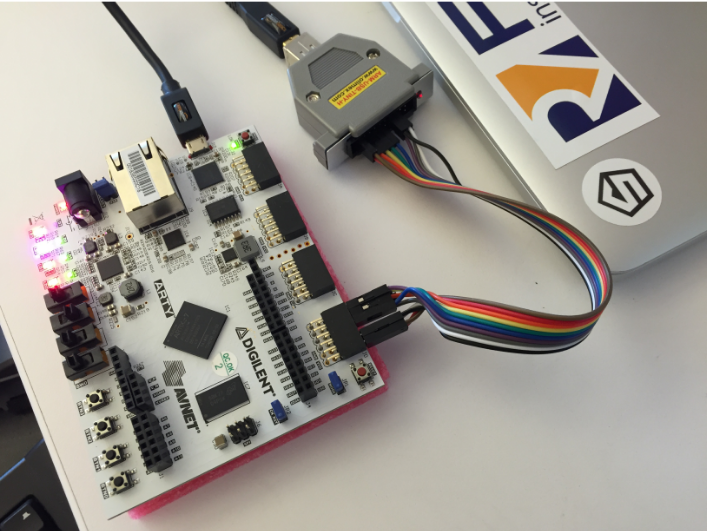
\includegraphics[width=0.7\linewidth]{./OlimexSetup.png}
  \caption{Olimex Debugger Setup~\cite[p.~5]{FreedomDevGuide}}
  \label{fig:olimexsetup}
\end{figure}

\section{Customizing an FPGA Image}\label{sec:Customizing}
In Chipyard, the directory used for all FPGA prototyping functionality is \mintinline{bash}{/fpga}, located in the root directory. 
Inside this directory there are several important files.

\subsection{Makefile}
Inside the Makefile is where you are able to define a custom Subproject as shown in \Cref{subsec:Makefile_SUB_PROJECT}. 
This allows users to control what files are compiled and generated for the FPGA Image. 
This is highly recommended as it simplifies the workflow for repeated compilation attempts.

\subsection{Configuration Directory}
The configuration directory for the Arty FPGA is located under \file{/src/main/scala/arty/}. 
This directory includes several useful files, including \file{Configs.scala}, \file{HarnessBinders.scala}, \file{IOBinders.scala}, and \file{TestHarness.scala}.

\subsubsection{Configs.scala}
This file is where 

\subsubsection{HarnessBinders.scala}
This file is where 

\subsubsection{IOBinders.scala}
This file is where 

\subsubsection{TestHarness.scala}
This file is where 

\subsection{Generated-src Directory}

\section{Generating the FPGA Image}
\subsection{Syntax}


\section{Using the FPGA Image}
\subsection{Flashing the Image}
\subsection{Uploading Programs to the FPGA}
%%% Local Variables:
%%% mode: latex
%%% TeX-master: "../doc"
%%% End:
